\documentclass{article}
\usepackage[utf8]{inputenc}
\usepackage{listings}
\usepackage{graphicx}
\usepackage{float}

\setlength{\parindent}{0pt}
\lstset{
    basicstyle=\ttfamily\footnotesize,
    frame=single,
    xleftmargin=4pt,
    xrightmargin=4pt,
    breaklines=true
}

\title{Lab Report: Particle Argon Peripherals}
\author{Lue Xiong}

\begin{document}

\maketitle
\newpage
\obeylines

\section{Introduction}
The focus of the lab is to gain understanding of circuits and how current flow sthroughout a given breadboard schematic with different electrical components such as sensors and peripherals. The lab also shows how these electrical components might be used in isolation as well as in combination with each other; denoting some sense of real-world application. Secondary to this is how a breadboard interacts with the given electrical components, and how to compose them together.

\section{Problem Statement}
The lab can be summarized down to five main different parts, which include:

\begin{itemize}
\item RGB LED -- Utilize Particle Argon's pulse-width modulation capability on pins \textit{D2}, \textit{D3}, and \textit{D4}
\item Piezzo Buzzer -- Modify the code to play the same sequence as the “two-bits.mp4”
\item Switches -- Explain the difference between \textbf{mom = 0} and \textbf{mom = 1} in relation to the momentary switch being depressed as well as the minimum voltage required for \textbf{mom = 1}
\item Servo -- Modify the code to reset when the servo rotation passes 180 degrees, rotating at 20 degrees increment when the momentary switch is depressed. Then publish each incremental reset to an IoT cloud platform
\item Analog Temperature Sensor -- Convert the ADC values to celsius and fahrenheit values and publish them as separate events to an IoT cloud platform.
\end{itemize}

\section{Process}
\subsection{Part One: RGB LED}
\begin{figure}[H]
\center
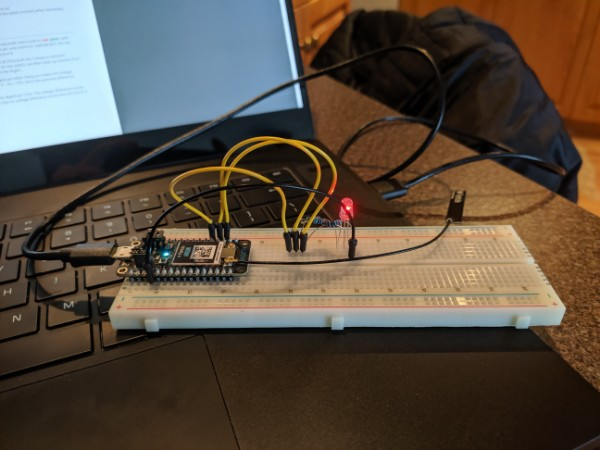
\includegraphics[width=\textwidth]{images/fade.jpeg}
\caption{Particle Argon RGB LED}
\label{fig:fade}
\end{figure}

The code below shows how to create the fade effect on the RGB LED by using a function called \textbf{fade()}. The function starts with a loop that increments \textit{brightness} by 1 from 0 to 255 with 10 millisecond delays in between. Upon reaching \textit{brightness} value 255, another loop will run and decrement by 1 from 255 to 0 with 10 millisecond delays in between. It is in practice, a rather slow fade but it works nonetheless. Figure~\ref{fig:fade} is a photo of the components composition on the breadboard.

\begin{minipage}[c]{\textwidth}
\lstinputlisting[language=C]{../archive/rgb-led.ino}
\end{minipage}

\subsection{Part Two: Piezzo Buzzer}
\begin{figure}[H]
\center
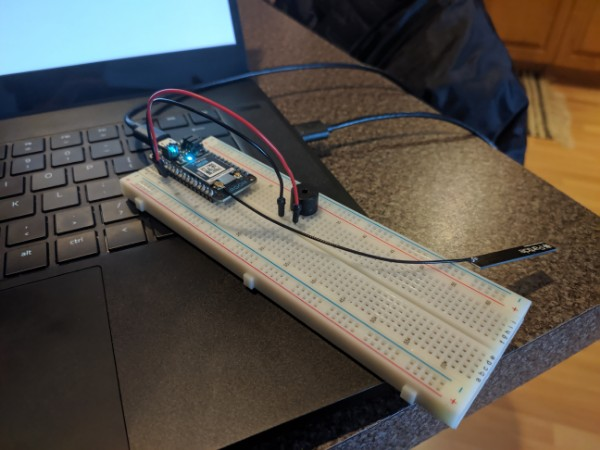
\includegraphics[width=\textwidth]{images/buzzer.jpeg}
\caption{Particle Argon Piezzo Buzzer}
\label{fig:buzzer}
\end{figure}

The code below shows how to create the two-bits sound on the piezzo buzzer by using a function called \textbf{twoBitsBuzz()}. The function sends currents of multiple levels to the piezzo buzzer at arbritrary times in attempt to mimic the "two-bits.mp4" tune. Figure~\ref{fig:fade} is a photo of the components composition on the breadboard.

\begin{minipage}[c]{\textwidth}
\lstinputlisting[language=C]{../archive/piezzo-buzzer.ino}
\end{minipage}

\subsection{Part Three: Switches}
\begin{figure}[H]
\center
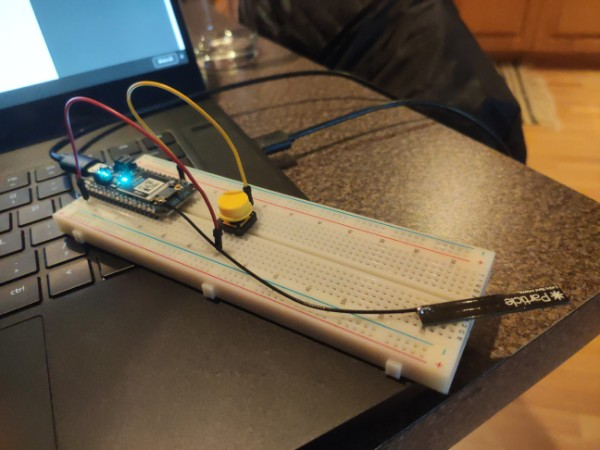
\includegraphics[width=\textwidth]{images/switches.jpeg}
\caption{Particle Argon Switches}
\label{fig:switches}
\end{figure}

When the momentary switch is depressed, it engages metal to metal contact which creates a circuit for currents to run through. When it is released from being depressed, the circuit is broken. In this context, assuming the momentary switch is depressed, 3.3 volts will flow from the \textbf{3V3} pin to the \textbf{D2} pin and keep looping as such. Essentially this is what happens when \textbf{mom = 1}.\\

\begin{figure}[H]
\center
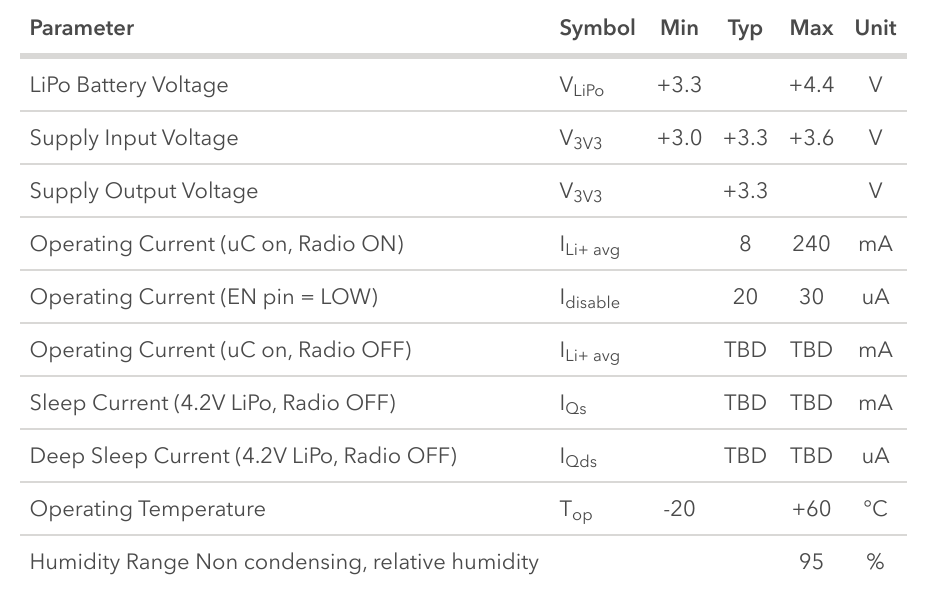
\includegraphics[width=\textwidth]{images/operating-conditions.png}
\caption{Particle Argon Operating Conditions}
\label{fig:operating}
\end{figure}

As shown on Figure~\ref{fig:operating} -- more specifically the \textbf{Supply Input Voltage} parameter -- the minimum voltage stated is 3.0 volts for inputs like momentary switches. Interestingly enough, the maximum voltage is 3.6 volts, which means that there is a +/- 0.3 volt difference from the typical 3.3 volt.\\

\begin{minipage}[c]{\textwidth}
\lstinputlisting[language=C]{../archive/switches.ino}
\end{minipage}\ \\

The code above produces the outputs on the serial monitor in Figure~\ref{fig:mom}. The \textbf{mom = 0} state means that there is no physical connection between the \textbf{3V3} and \textbf{D2} pin. The \textbf{mom = 1} means that the momentary switch is depressed to create a physical connection between \textbf{3V3} and \textbf{D2} pin.

\begin{figure}[H]
\center
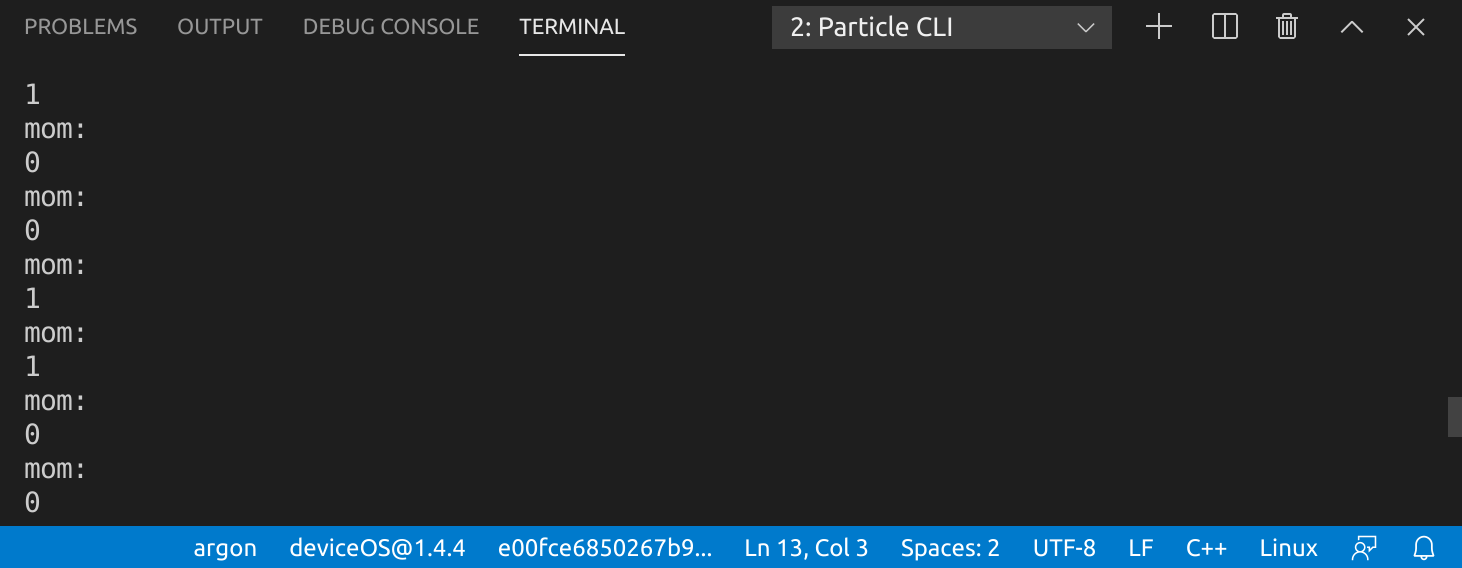
\includegraphics[width=\textwidth]{images/mom.png}
\caption{Particle Argon Switches}
\label{fig:mom}
\end{figure}

\subsection{Part Four: Servo}
\begin{figure}[H]
\center
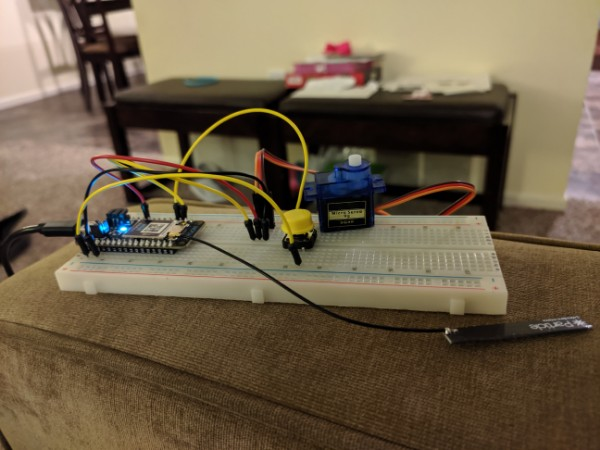
\includegraphics[width=\textwidth]{images/servo.jpeg}
\caption{Particle Argon Servo}
\label{fig:servo}
\end{figure}

The code below shows how to rotate the servo from 0 to 181 degrees with 20 degrees rotation per button depression. Upon reaching any value greater than 180, the servo will reset itself to 0 degrees and publishes a reset counter to Particle Cloud. The reset counter increments for every time the servo resets to 0 degrees.\\

\begin{minipage}[c]{\textwidth}
\lstinputlisting[language=C]{../archive/servo.ino}
\end{minipage}\ \\

Figure~\ref{fig:events} shows reset counters published to Particle Cloud. Figure~\ref{fig:resetCounter} is a follow-up with a webhook to capture the value to the Losant IoT platform.

\begin{figure}[H]
\center
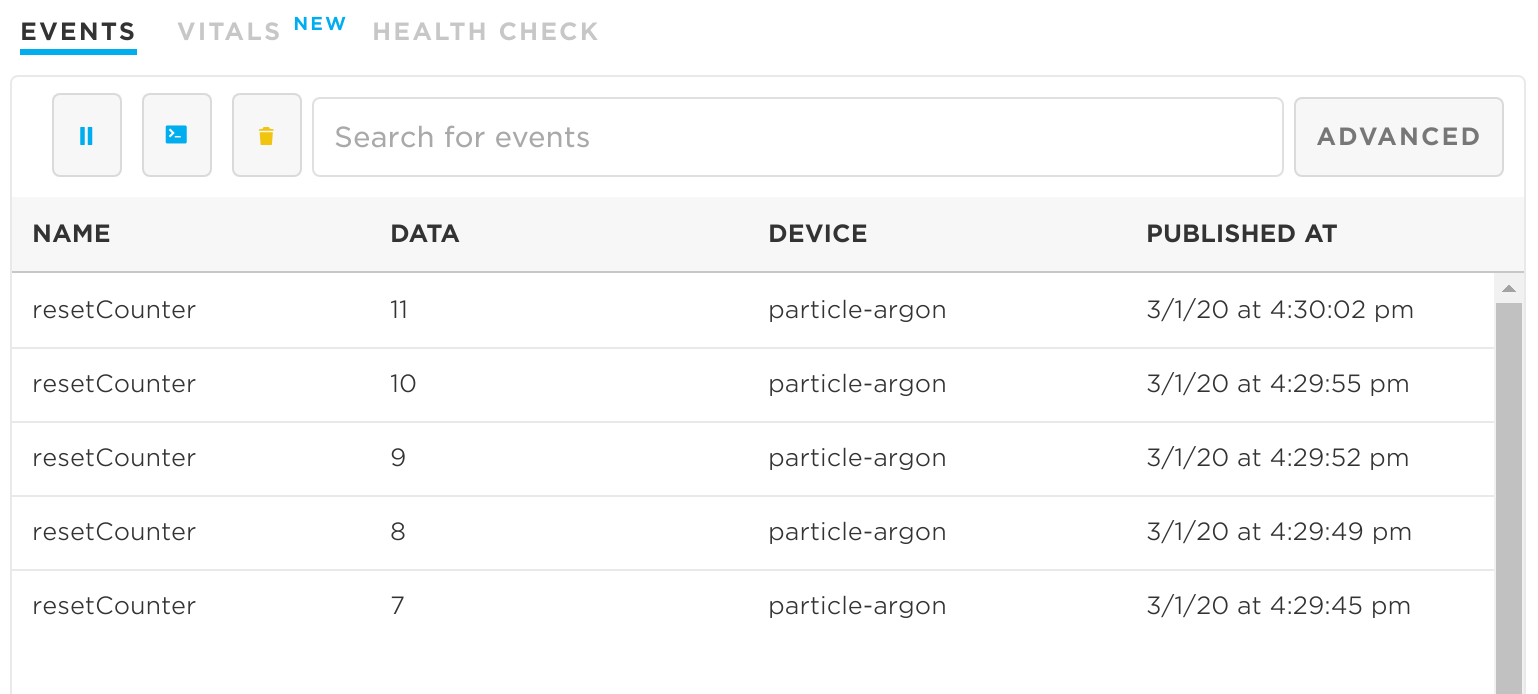
\includegraphics[width=\textwidth]{images/events.png}
\caption{Particle Argon Cloud Events}
\label{fig:events}
\end{figure}

\begin{figure}[H]
\center
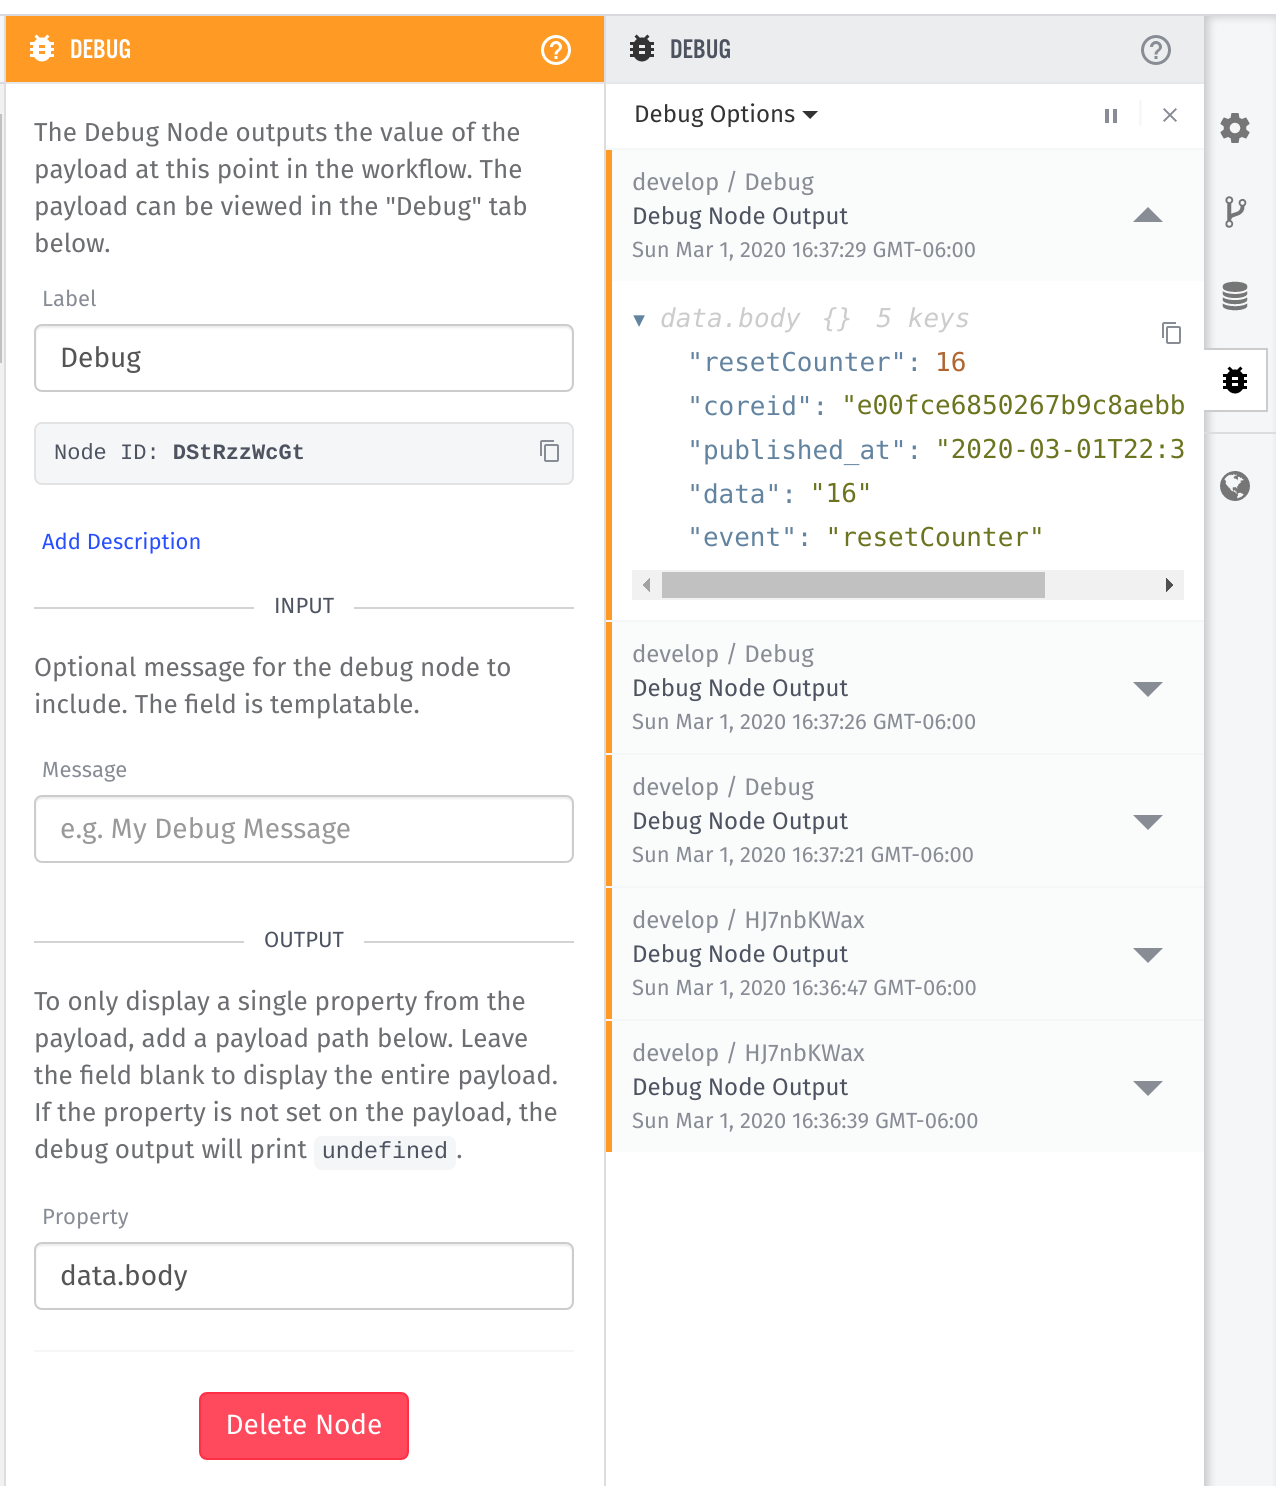
\includegraphics[width=.8\textwidth]{images/resetCounter.png}
\caption{Particle Argon Reset Counter}
\label{fig:resetCounter}
\end{figure}

\subsection{Part Five: Thermistor}
\begin{figure}[H]
\center
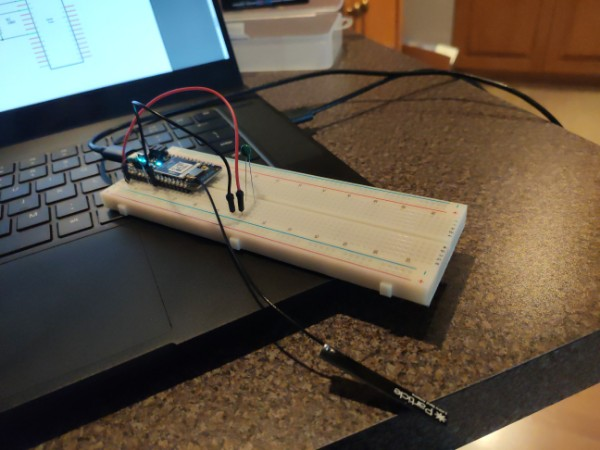
\includegraphics[width=\textwidth]{images/temperature.jpeg}
\caption{Particle Argon Thermistor}
\label{fig:temperature}
\end{figure}\ \\

The code below calulates ADC values into celsius and fahrenheit values. The main equation used was the Steinhart and Hart equation for NTC thermistors, which is mathematically represented as such:

\[T=\frac{1}{A+B \ln (R)+C[\ln (R)]^{3}}\]

\textbf{T} in the equation represents temperature in celsius degrees. In order to convert from celsius to fahrenheit degrees, the following mathematical forumla was used:

\[T_{\left(^{\circ} \mathrm{F}\right)}=T_{\left(^{\circ} \mathrm{C}\right)} \times 9 / 5+32\]

\begin{minipage}[c]{\textwidth}
\lstinputlisting[language=C]{../archive/thermistor.ino}
\end{minipage}\ \\

Both of these formulas are represented in C code. After the calculations are made, they are both published as events shown in Figure~\ref{fig:temperaturevalues} and then separated to two different channels to be displayed on graphs. The graphs can be found in Figure~\ref{fig:temperaturegraphs}.
\begin{figure}[H]
\center
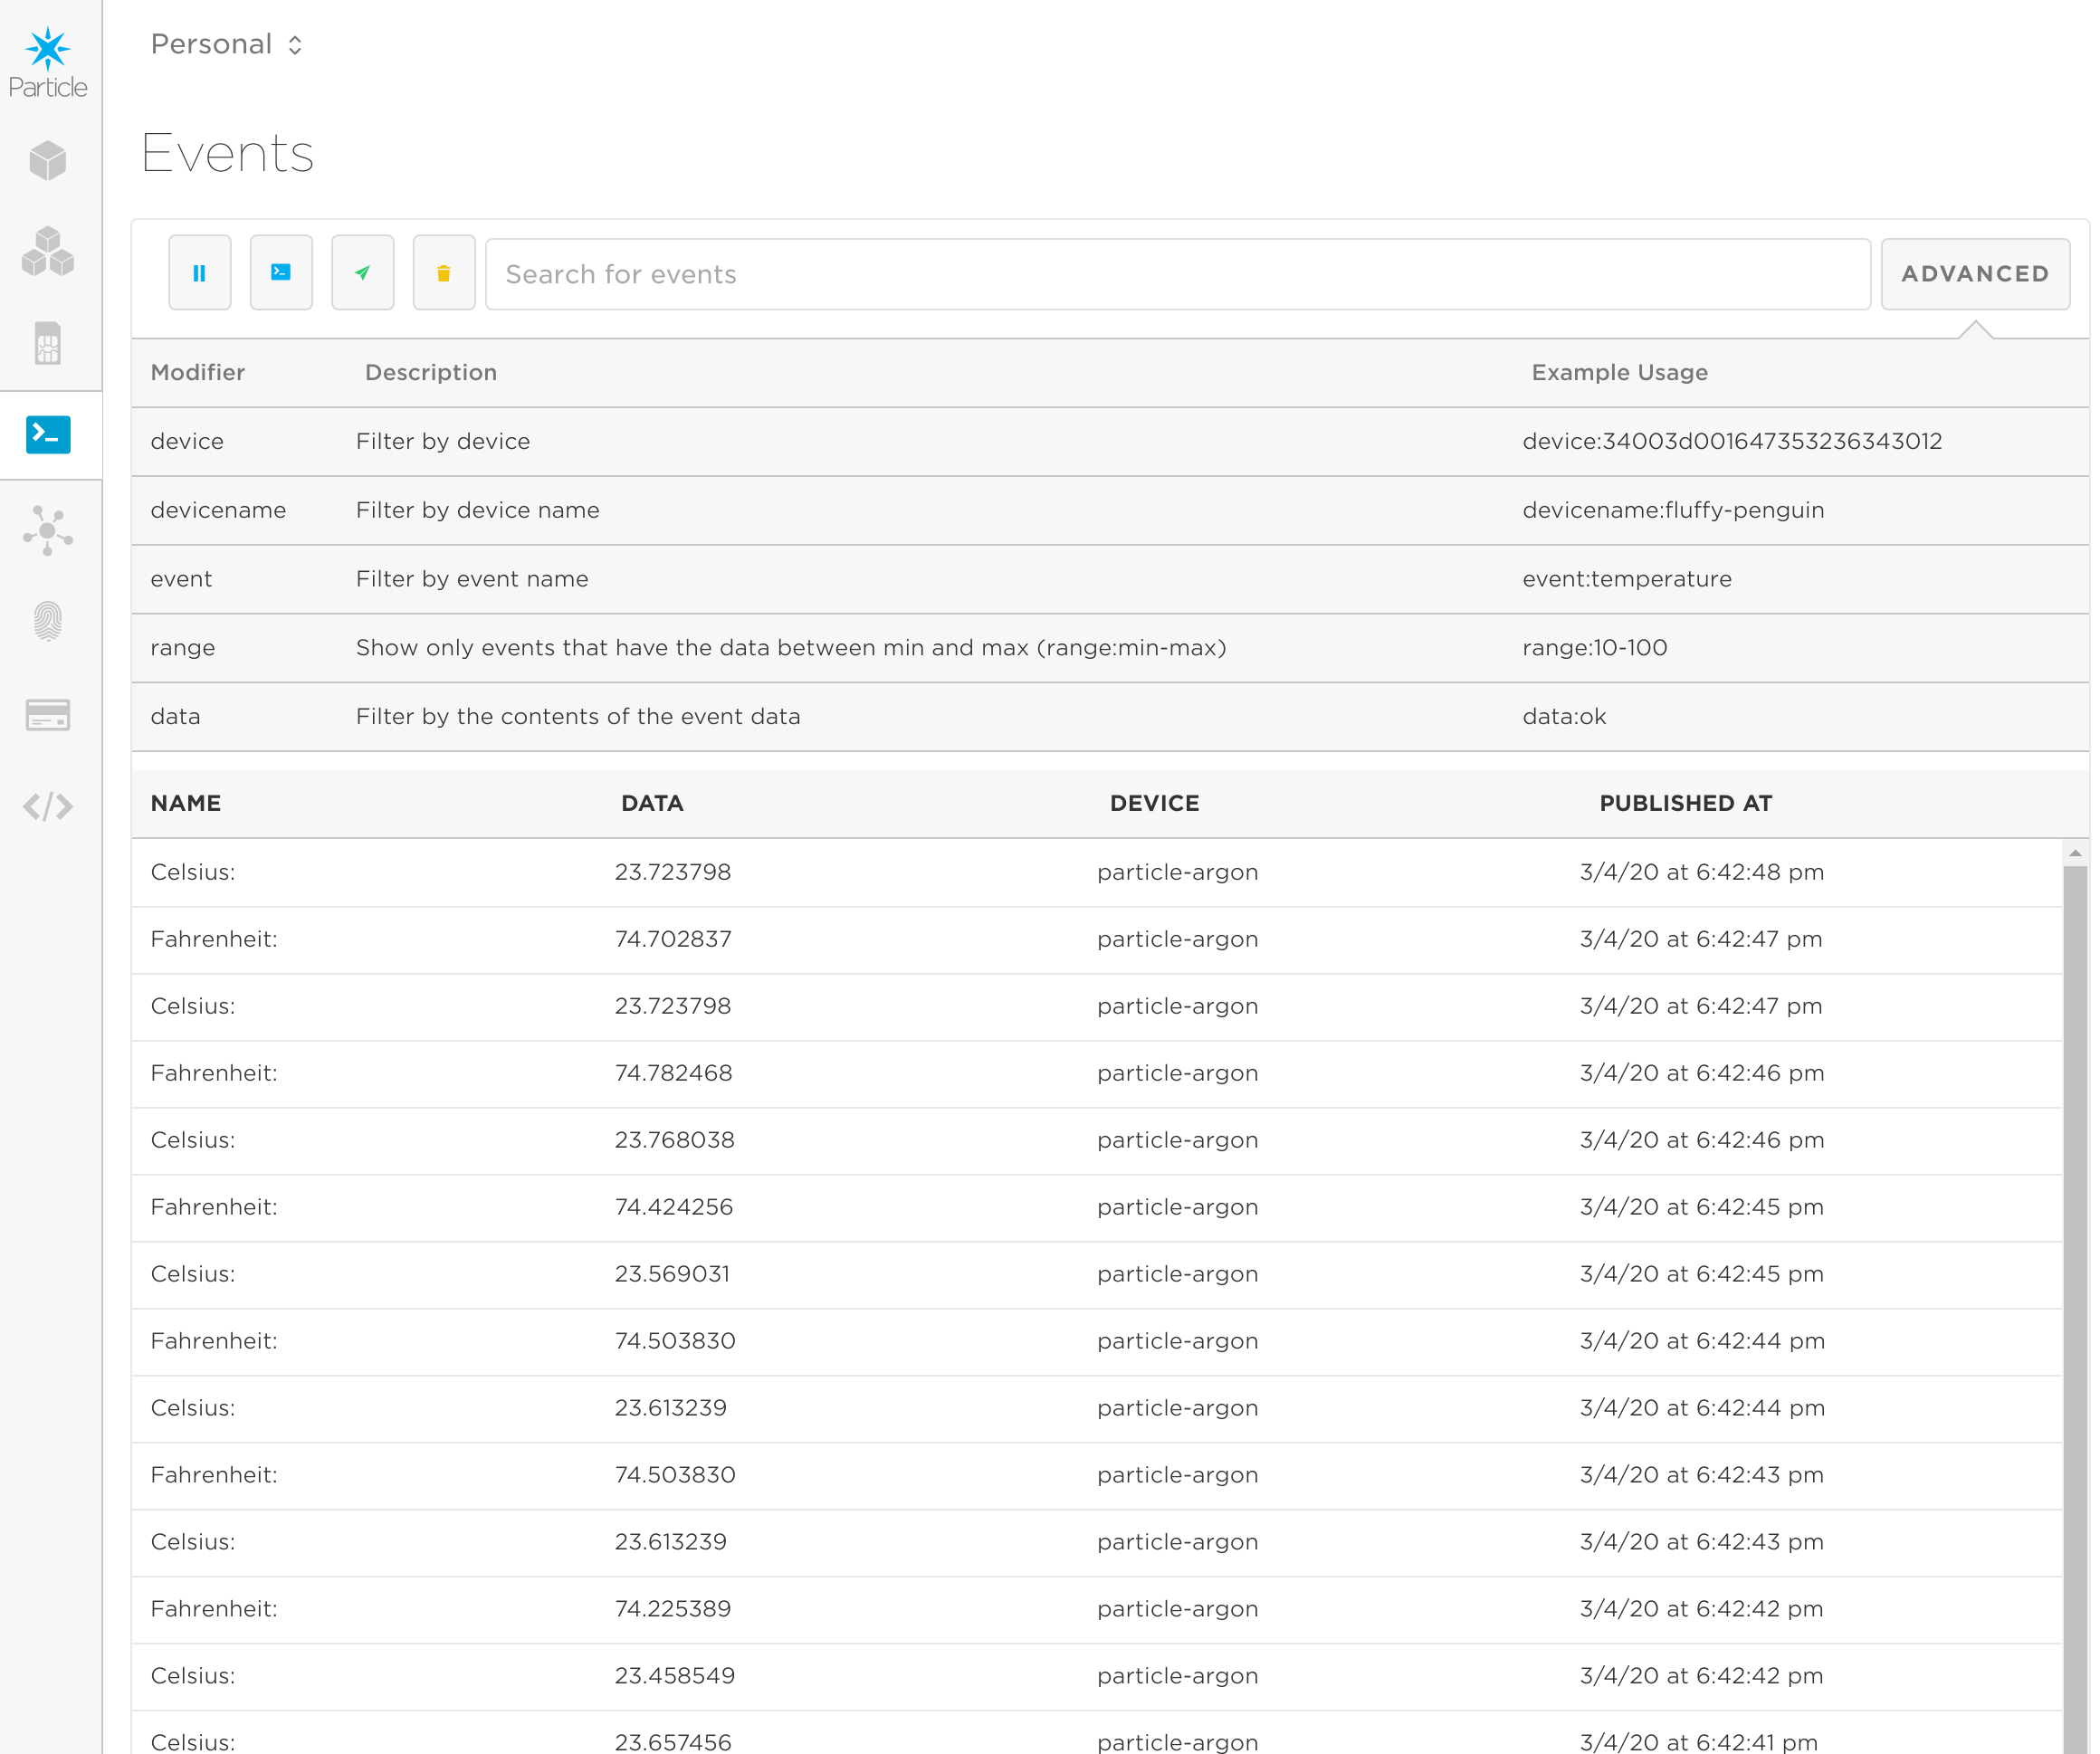
\includegraphics[width=\textwidth]{images/celsius-fahrenheit.png}
\caption{Particle Argon Celsius and Fahrenheit}
\label{fig:temperaturevalues}
\end{figure}

\begin{figure}[H]
\center
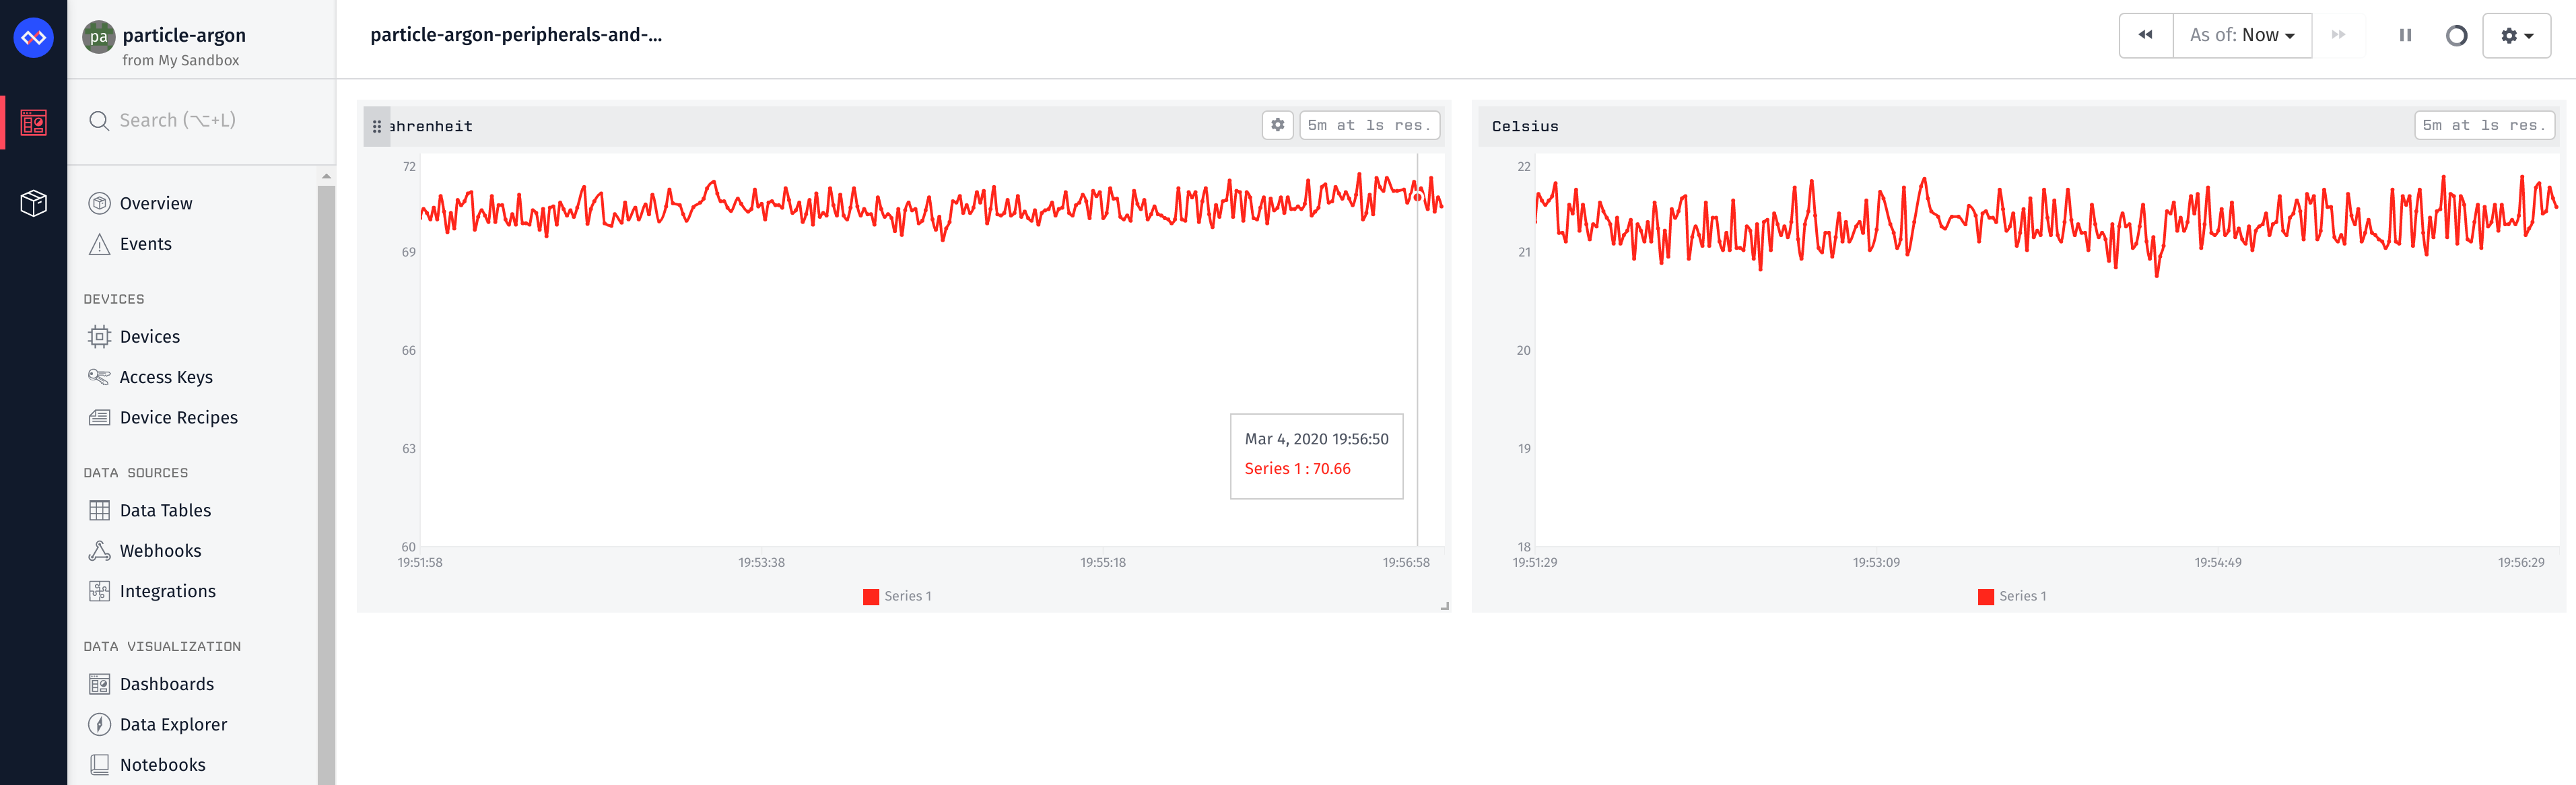
\includegraphics[width=\textwidth]{images/celsius-fahrenheit-graphs.png}
\caption{Particle Argon Celsius and Fahrenheit Graphs}
\label{fig:temperaturegraphs}
\end{figure}

\newpage

\section{Discussion of Results}
Part five of the lab concerning temperature were the most difficult because there were many unfamiliar formulas in addition to having to do mathematics in general. The results were however satisfactory as they fit real world numbers that would be measured with either a temperature sensor or thermometer. Part two concerning the piezzo buzzer was the most interesting because all of the buzzes were the same pitch. It was also hard to decipher the time gaps in between each buzz to recreate the "two-bits.mp4" melody. The least interesting was the momentary switch as it was a matter of on or off; though I see can this being very practical to use for everyday convenience, such as a remote control.

\section{Conclusion}
The lab was a good learning experience being that there were a variety of electrical components to manipulate. Applying how the ground pin relates to the voltage pin with currents circulating to each electrical component also cemented the idea of how eletric works. It is enlightening to experience the practicality and usefulness of the breadboard. Not having to solder metal together and just having things work on the breadboard makes this lab very convenient. I will say however, that my bias favored me torwards the coding portion of the lab, since I am a software engineer at heart.

\end{document}
